\section{Experimental Analysis}
\label{exp: dtr}

\begin{table*}[ht!]\scriptsize
\centering
\caption{Comparisons over the RealHitBench dataset for five different task types.}
\resizebox{0.98\textwidth}{!}{%
\begin{tabular}{@{}l|cc|cc|cc|cc|ccc@{}}
\toprule
\multirow{3}{*}{\textbf{Methods}}

& \multicolumn{2}{c}{\makecell{\textbf{Fact}\\\textbf{Checking}}} & \multicolumn{2}{c}{\makecell{\textbf{Numerical}\\\textbf{Reasoning}}} & \multicolumn{2}{c}{\makecell{\textbf{Structure}\\\textbf{Comprehending}}} & \multicolumn{2}{c}{\makecell{\textbf{Data}\\\textbf{Analysis}}} & \multicolumn{2}{c}{\makecell{\textbf{Chart/Report}\\\textbf{Generation}}} \\
\cmidrule(lr){2-3} \cmidrule(lr){4-5} \cmidrule(lr){6-7} \cmidrule(lr){8-9} \cmidrule(lr){10-11}
& EM$\uparrow$ & F1$\uparrow$ & EM$\uparrow$ & F1$\uparrow$ & EM$\uparrow$ & F1$\uparrow$ & \makecell{LLM-EVAL}$\uparrow$ & ROUGE$\uparrow$ & \makecell{PASS@1}$\uparrow$ & ECR$\uparrow$ \\
\midrule
TableGPT2-7B & 46.10 & 53.80 & 29.31 & 39.81 & 48.23 & 56.68 & 62.76 & 33.25 & 32.47 & 67.53 \\
TableLLM-7B & 38.25 & 44.12 & 22.40 & 31.65 & 41.10 & 49.34 & 55.80 & 28.42 & 18.20 & 42.15 \\
StructGPT & 25.40 & 32.15 & 14.55 & 20.80 & 30.25 & 38.60 & 42.33 & 19.50 & 5.12 & 12.44 \\
\midrule
GPT4o & 43.39 & 51.87 & 27.63 & 36.68 & 42.68 & 52.89 & 65.24 & 33.10 & 10.39 & 25.32 \\
DeepSeek-v3 & 57.21 & 53.42 & 47.05 & 50.61 & 43.31 & 74.63 & 61.40 & 34.76 & 9.09 & 24.68 \\
\midrule
Code Loop (DeepSeek-v3) & 48.19 & 56.49 & 42.93 & 49.68 & 44.19 & 51.95 & 62.51 & 33.73 & 20.78 & 39.60 \\
% Code Loop (Youtu-LLM-2B) & 6.00 & 7.01 & 3.50 & 5.05 & 15.15 & 22.07 & 17.33 & 15.92 & 0.00 & 0.00 \\
Code Loop (Qwen3-1.7B) & 6.91 & 7.65 & 4.02 & 5.75 & 49.24 & 53.08 & 17.97 & 17.29 & 0.00 & 0.60 \\
Code Loop (Qwen3-4B) & 16.61 & 19.76 & 10.25 & 13.00 & 32.85 & 30.30 & 25.83 & 18.17 & 3.25 & 14.30 \\
% \midrule

\midrule
\midrule
% DTR (Youtu-LLM-2B) & 11.42 & 16.09 & 4.54 & 10.97 & 5.81 & 23.00 & 20.07 & 13.40 & 1.30 & 14.84 \\
DTR (Qwen3-1.7B) & 17.93 & 23.50 & 13.75 & 19.01 & 17.17 & 27.88 & 40.28 & 16.44 & 5.16 & 21.94 \\
DTR (Qwen3-4B) & 30.42 & 37.44 & 22.05 & 30.13 & 32.6 & 43.32 & 53.88 & 20.15 & 8.39 & 30.32 \\
DTR (DeepSeek-v3) &\textbf{58.22} &\textbf{64.47} &\textbf{55.51} &\textbf{61.98} &\textbf{56.57} &\textbf{77.95} &\textbf{70.90} &\textbf{38.67} &\textbf{52.69} & \textbf{100.00} \\							
\bottomrule
\end{tabular}%
\label{exp: real}
}
\end{table*}

We evaluate Deep Tabular Research (DTR) on a diverse set of unstructured tabular reasoning benchmarks, covering factual lookup, numerical computation, structural understanding, long-horizon data analysis, and visualization tasks. 
Our evaluation focuses on both \emph{task accuracy} and \emph{end-to-end analytical effectiveness}, reflecting the real-world demands of complex spreadsheet-based workflows. The details of the adopted benchmarks, state-of-the-art baselines and evaluation protocols are introduced in Appendix~\ref{implement}.

% \subsection{Benchmark Datasets}
% \label{sec:datasets}

% \paragraph{DTR-Bench: Long-Horizon Analytical Queries.}
% To profoundly evaluate the performance for complex and long-horizon tabular reasoning datasets, we construct an additional DTR-Bench based on tables in RealHitBench. Using table meta information and expert-designed templates combined with \texttt{DeepSeek-3.2}, we generate 500 long-form analytical queries that require multi-step reasoning and execution. These queries span five categories: \textit{Analysis}: multi-stage aggregation and interpretation. \textit{Visualization}: chart generation and visual comparison. \textit{Calculation}: chained numerical computation. \textit{Comparison}: cross-group or temporal comparison. \textit{Conditional Calculation}: conditional aggregation and filtering.

% Each query typically requires planning over multiple operations and intermediate execution states, making them unsuitable for shallow or single-pass reasoning approaches.

% For the evaluation, we report two following metrics. \textit{Win Rate}: proportion of instances where a model outperforms baselines (ties counted as $0$). \textit{Score Rate}: proportion of instances where a model is not worse than baselines (ties counted as $0.5$).


% \paragraph{RealHitBench.}
% We adopt RealHitBench~\cite{wu2025realhitbench} as our primary benchmark, a large-scale dataset designed for evaluating reasoning over real-world, unstructured tables.
% RealHitBench contains tables with heterogeneous layouts, including merged cells, bidirectional and hierarchical headers, missing values, and implicit semantic regions.
% The benchmark categorizes tasks into multiple reasoning types and provides fine-grained evaluation protocols.

% We evaluate DTR on the following RealHitBench task categories: \textit{Fact Checking}: verifying factual statements grounded in table entries. \textit{Numerical Reasoning}: performing arithmetic and aggregation over table values. \textit{Structure Comprehension}: understanding table organization, header hierarchy, and alignment. \textit{Data Analysis}: multi-step analytical reasoning requiring aggregation, comparison, and synthesis. \textit{Visualization}: generating charts or structured visual outputs based on tabular data.


% For Fact Checking, Numerical Reasoning, and Structure Comprehension, we report \textit{Exact Match (EM)} and \textit{F1} scores following the benchmark protocol.
% Data Analysis tasks are evaluated using \textit{LLM-based evaluation} and \textit{ROUGE} metrics to assess semantic correctness and completeness.
% Visualization tasks are evaluated using \textit{Execution Correctness Rate (ECR)} and \textit{Pass@1}, measuring whether the generated visualization code executes successfully and produces the expected output.


% \subsection{Baselines}
% \label{sec:baselines}

% We compare DTR against a diverse set of baselines spanning table-specialized models, general-purpose large language models, and agent-based reasoning frameworks. 
% \textbf{Table-specific Models.} TableGPT~\cite{gong2020tablegpt}: a representative table-focused language model designed for structured table question answering. \textbf{General-purpose LLMs.} DeepSeek-3.2: a strong open-source large language model with competitive reasoning capabilities; \textbf{Agentic Frameworks.} ST-RAPTOR~\cite{tang2025st}: a retrieval-augmented agent framework for structured reasoning; Tree Thinker~\cite{wu2025realhitbench}: a tree-based reasoning agent that explores multiple reasoning branches; CodeLoop: we craft a straightforward execution-centric agentic framework that iteratively generates and debugs code. All baselines are evaluated under comparable settings, with access to the same table inputs and query information.
% Unless otherwise specified, we use publicly released model checkpoints and default decoding configurations.

\subsection{Main Results}
Tables~\ref{exp: dtr} and Table~\ref{exp: real} report the main experimental results on DTR-Bench and RealHitBench, respectively. Though both benchmarks target table-centric reasoning, they emphasize fundamentally different aspects of model capability. For fair comparison, we allow non-code mode for the RealHitBench dataset since it focuses on answer-level correctness with concise formats. On DTR-Bench, DTR achieves the strongest overall performance across all dimensions, including accuracy, analysis depth, feasibility, and aesthetics. Notably, the improvements are consistent under both strict win-rate and more tolerant score-rate evaluation, indicating that DTR does not merely outperform baselines in marginal cases, but produces systematically higher-quality outputs.

These gains cannot be attributed solely to stronger backbone models. Compared to pure LLM baselines, DTR demonstrates substantially deeper analysis and higher feasibility. This suggests that unconstrained language generation, even in large models, has difficulty reliably organizing multi-step table operations into executable workflows. Conversely, agent-based frameworks such as ST-Raptor, TreeThinker, and Code Loop exhibit improved structural reasoning but incur significant computational overhead and instability due to extensive branching and repeated trial executions. DTR stands out in this trade-off space. By explicitly planning over macro-level operation paths and selecting candidates based on learned expectations derived from historical experience, DTR avoids exhaustive search while still preserving long-range reasoning coherence. As a result, it produces more complete and visually coherent analytical reports than pure LLMs, while remaining substantially more efficient than tree-based or loop-based agent frameworks.

Beyond quality, DTR also demonstrates favorable efficiency–performance balance. While workflow-based baselines often require an order of magnitude more LLM calls and runtime to achieve competitive analytical depth, DTR attains superior results with fewer calls and more predictable execution cost. This suggests that reasoning at the level of operation sequences, rather than token-level or step-level exploration, leads to more stable and scalable analytical behavior for complex table reasoning tasks.

\begin{table}[ht!]
\centering
\caption{Architecture ablation study of each components in DTR.}
\label{tab:architecture_ablation}
\resizebox{\linewidth}{!}{%
\begin{tabular}{lcccccccc}
\toprule
\textbf{Configuration} & \textbf{Meta} & \textbf{QDO} & \textbf{Exp.} & \textbf{Abst.} & \textbf{Acc.} & \textbf{Anal.} & \textbf{Feas.} & \textbf{Aesth.} \\
\midrule
+ Meta Info & \checkmark & $\times$ & $\times$ & $\times$ & 34.8 & 27.1 & 25.6 & 38.2 \\
+ QDO & \checkmark & \checkmark & $\times$ & $\times$ & 36.2 & 28.8 & 26.7 & 40.5 \\
+ Expectation & \checkmark & \checkmark & \checkmark & $\times$ & 37.1 & 29.6 & 27.2 & 41.8 \\
\textbf{DTR Full} & \checkmark & \checkmark & \checkmark & \checkmark & \textbf{37.5} & \textbf{30.2} & \textbf{27.6} & \textbf{42.7} \\
\bottomrule
\end{tabular}%
}
\vspace{-3mm}
\end{table}

\subsection{Ablation Studies}
\label{sec:ablation}
\subsubsection{Component Contributions}
We conduct a systematic ablation study to quantify the marginal contribution of each constituent module within our framework. Beginning with a \textbf{pure LLM baseline} (DeepSeek-V3), we progressively integrate \((i)\) tabular meta information, \((ii)\) query-to-operation decomposition, \((iii)\) expectation-aware macro path selection informed by historical execution feedback, and \((iv)\) abstracted execution experience. Table~\ref{tab:architecture_ablation} summarizes the results across multiple evaluation dimensions, including Accuracy, Analysis Depth, Feasibility, Aesthetics, and the mean number of LLM calls.

The results demonstrate that DTR yields consistent performance gains over the baseline, achieving a total accuracy improvement of \textbf{4.0} percentage points (33.5\% $\rightarrow$ 37.5\%). Among the individual components, tabular meta-information and query decomposition provide the most significant uplift (+1.3 and +1.4 points, respectively), which suggests that explicit structural grounding and operation-level intent modeling are fundamental to unstructured tabular reasoning. The incorporation of historical feedback for macro path selection further enhances accuracy by 0.9 points, indicating that high-level planning benefits substantially from past experience even in the absence of low-level code simulations. Finally, the inclusion of abstracted execution experience provides an additional 0.4 point gain, validating the utility of distilling raw execution outcomes into reusable knowledge for novel problem instances.

% We observe diminishing returns as the system complexity increases. While each module contributes positive gains, the incremental improvements become smaller with additional components. This trend aligns with our objective of decoupling foundational capabilities, such as table comprehension and decomposition, from iterative refinement processes like experience-aware planning and memory abstraction.

\begin{table}[ht!]
\centering
\caption{Exploration over prompting strategy for think and code.}
\label{tab:prompt_ablation}
\resizebox{\linewidth}{!}{%
\begin{tabular}{lcccc}
\toprule
\textbf{Prompt Strategy} & \textbf{Accuracy} & \textbf{Analysis} & \textbf{Code Error} & \textbf{Avg} \\
& & \textbf{Depth} & \textbf{Rate} & \textbf{Calls} \\
\midrule
No [THINK] (Direct) & 35.2 & 27.8 & 42.3\% & 5.8 \\
Simple [THINK] Hint & 36.4 & 28.9 & 35.6\% & 5.2\\
\textbf{[THINK]+[CODE]} & \textbf{37.5} & \textbf{30.2} & \textbf{28.4\%} & \textbf{4.78}\\
Multi-stage Reflection & 37.2 & 29.8 & 26.1\% & 5.5 \\
\bottomrule
\end{tabular}%
}
\end{table}
\subsubsection{Prompting Strategy Analysis}
\label{sec:prompt-ablation}

We observe diminishing returns as the system complexity increases. While each module contributes positive gains, the incremental improvements become smaller with additional components. This trend aligns with our objective of decoupling foundational capabilities, such as table comprehension and decomposition, from iterative refinement processes like experience-aware planning and memory abstraction.Given DTR's step-wise paradigm, code reliability is critical to both correctness and computational efficiency. We therefore evaluate various strategies during the execution phase. Table~\ref{tab:prompt_ablation} compares four configurations, including direct code generation without explicit reasoning steps, a lightweight reasoning hint, our default structured [THINK]+[CODE] prompting mode, and a multi-stage reflection strategy.

The structured [THINK]+[CODE] scheme well balances between performance and efficiency. It attains the highest accuracy (37.5\%) and analysis depth (30.2) while simultaneously reducing the code error rate from 42.3\% to 28.4\% compared to the direct generation baseline. Furthermore, this approach optimizes the average number of LLM calls (4.78 versus 5.8), which implies that isolating semantic reasoning from code emission enhances execution stability and mitigates redundant retry cycles. Although multi-stage reflection achieves a slightly lower error rate (26.1\%), it introduces substantial runtime overhead (48.6s versus 42.1s), suggesting that additional reflection yield marginal benefits.
\vspace{-3mm}
\subsection{Efficiency and Scalability}
\vspace{-1mm}
\label{sec:efficiency}
\begin{figure}
    \centering
    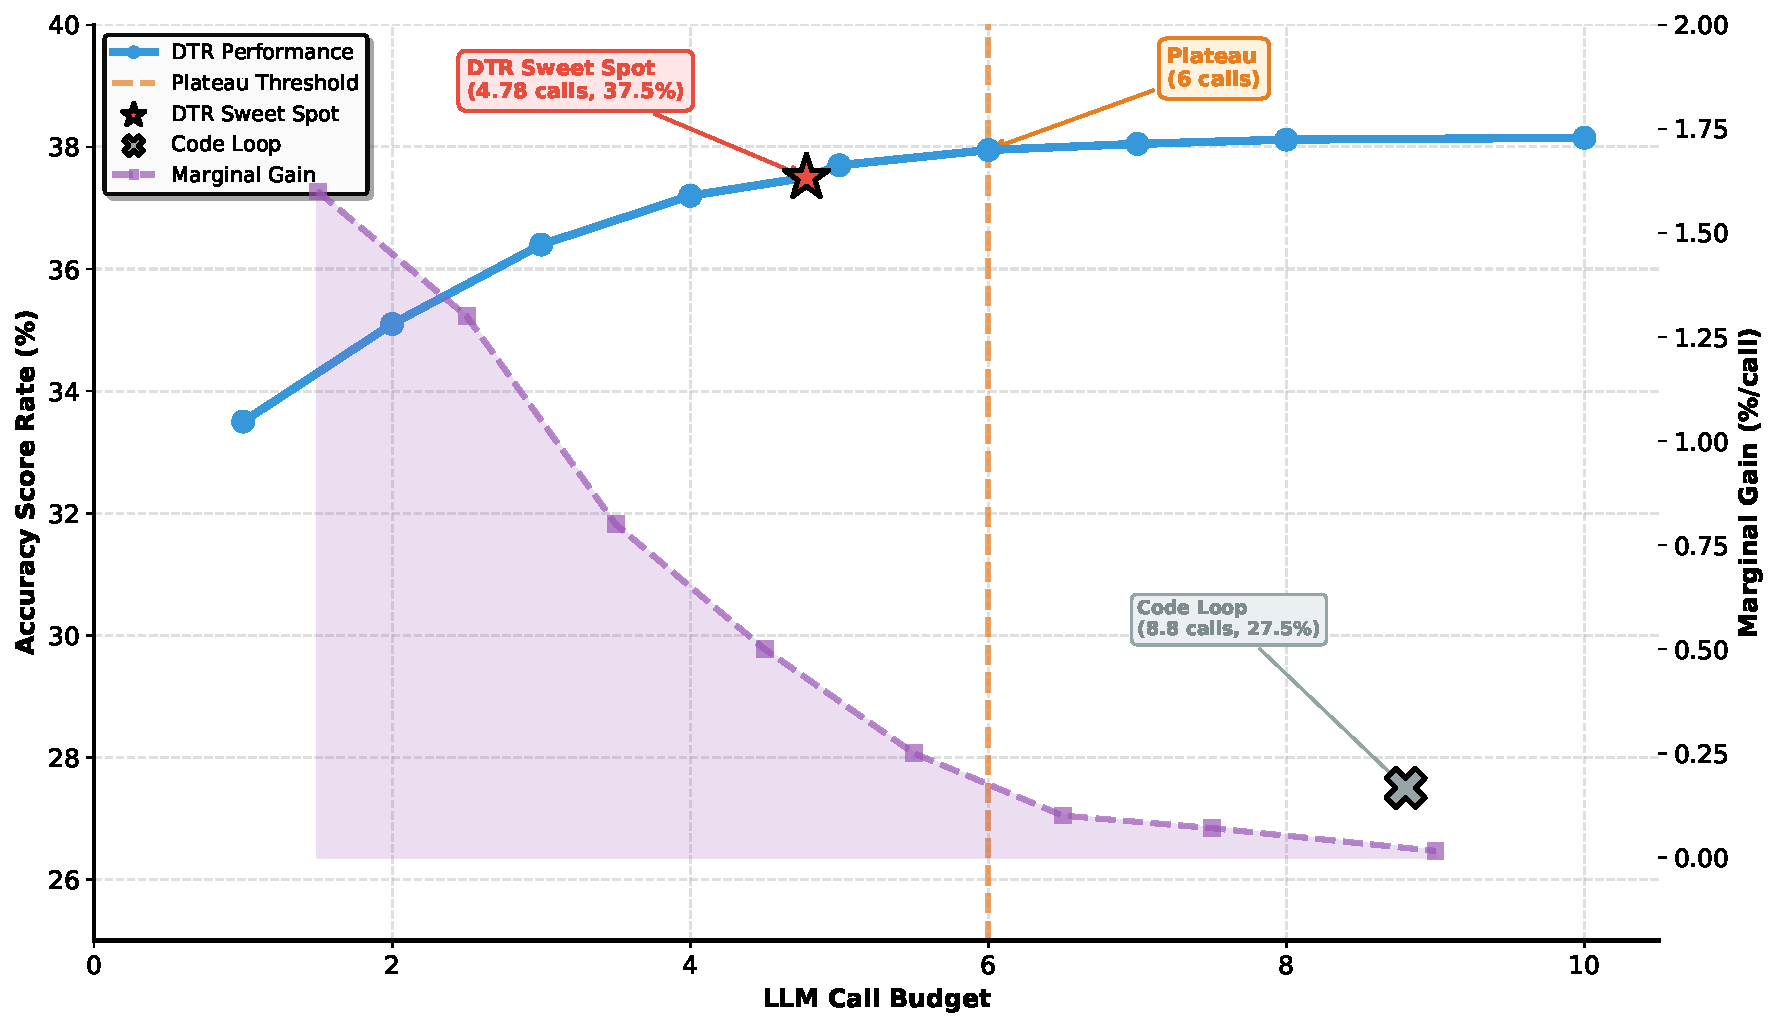
\includegraphics[width=0.85\linewidth]{resources/budget.pdf}
    \caption{\footnotesize LLM call budget analysis. The blue curve shows performance (left y-axis) and the purple curve shows marginal gain (right y-axis). DTR's 4.78-call configuration red star) achieves optimal efficiency by avoiding the plateau region.}
    \label{fig:budget}
\vspace{-6mm}
\end{figure}

We assess the computational efficiency of DTR by comparing model performance and the frequency of LLM calls, using the call budget as a proxy for inference-time cost. Figure~\ref{fig:budget} presents the performance trajectory as the budget increases and the marginal utility per additional call.

The analysis reveals three distinct regimes. In the rapid growth phase (1--3 calls), performance scales sharply with high marginal gains averaging approximately +1.45\% per call, demonstrating that even sparse iterative interactions significantly bolster long-horizon tabular reasoning. In the transitional regime (3--6 calls), improvements persist but decelerate to approximately +0.45\% per call as the system nears its performance ceiling. Beyond 6 calls, each additional call yields less than 0.15\% performance gain. DTR operates at an average of \textbf{4.78} calls, effectively positioning it within the optimal transition region where quality and computation are balanced. In contrast, the CodeLoop baseline exhibits a failure mode characterized by over-iteration. Despite exhausting a significantly higher budget (8.8 calls), it achieves only 27.5\% accuracy, suggesting that unconstrained execution without a strategic selection mechanism can propagate errors and degrade overall performance. These findings justify the importance of DTR’s budgeted design and its expectation-aware path selection.


% L→F→G	LOAD → FILTER → GROUPBY
% L→S→Se	LOAD → SORT → SELECT
% L→F→A	LOAD → FILTER → AGGREGATE
% L→G→A	LOAD → GROUPBY → AGGREGATE
% L→M→F	LOAD → MERGE → FILTER
% L→F→S	LOAD → FILTER → SORT
% L→Se→F	LOAD → SELECT → FILTER
% L→P→A	LOAD → PIVOT → AGGREGATE

\vspace{-1mm}
\subsection{Case Study: Planning Dynamics}
\vspace{-1mm}
\label{sec:case-study}
\begin{figure}
    \centering
    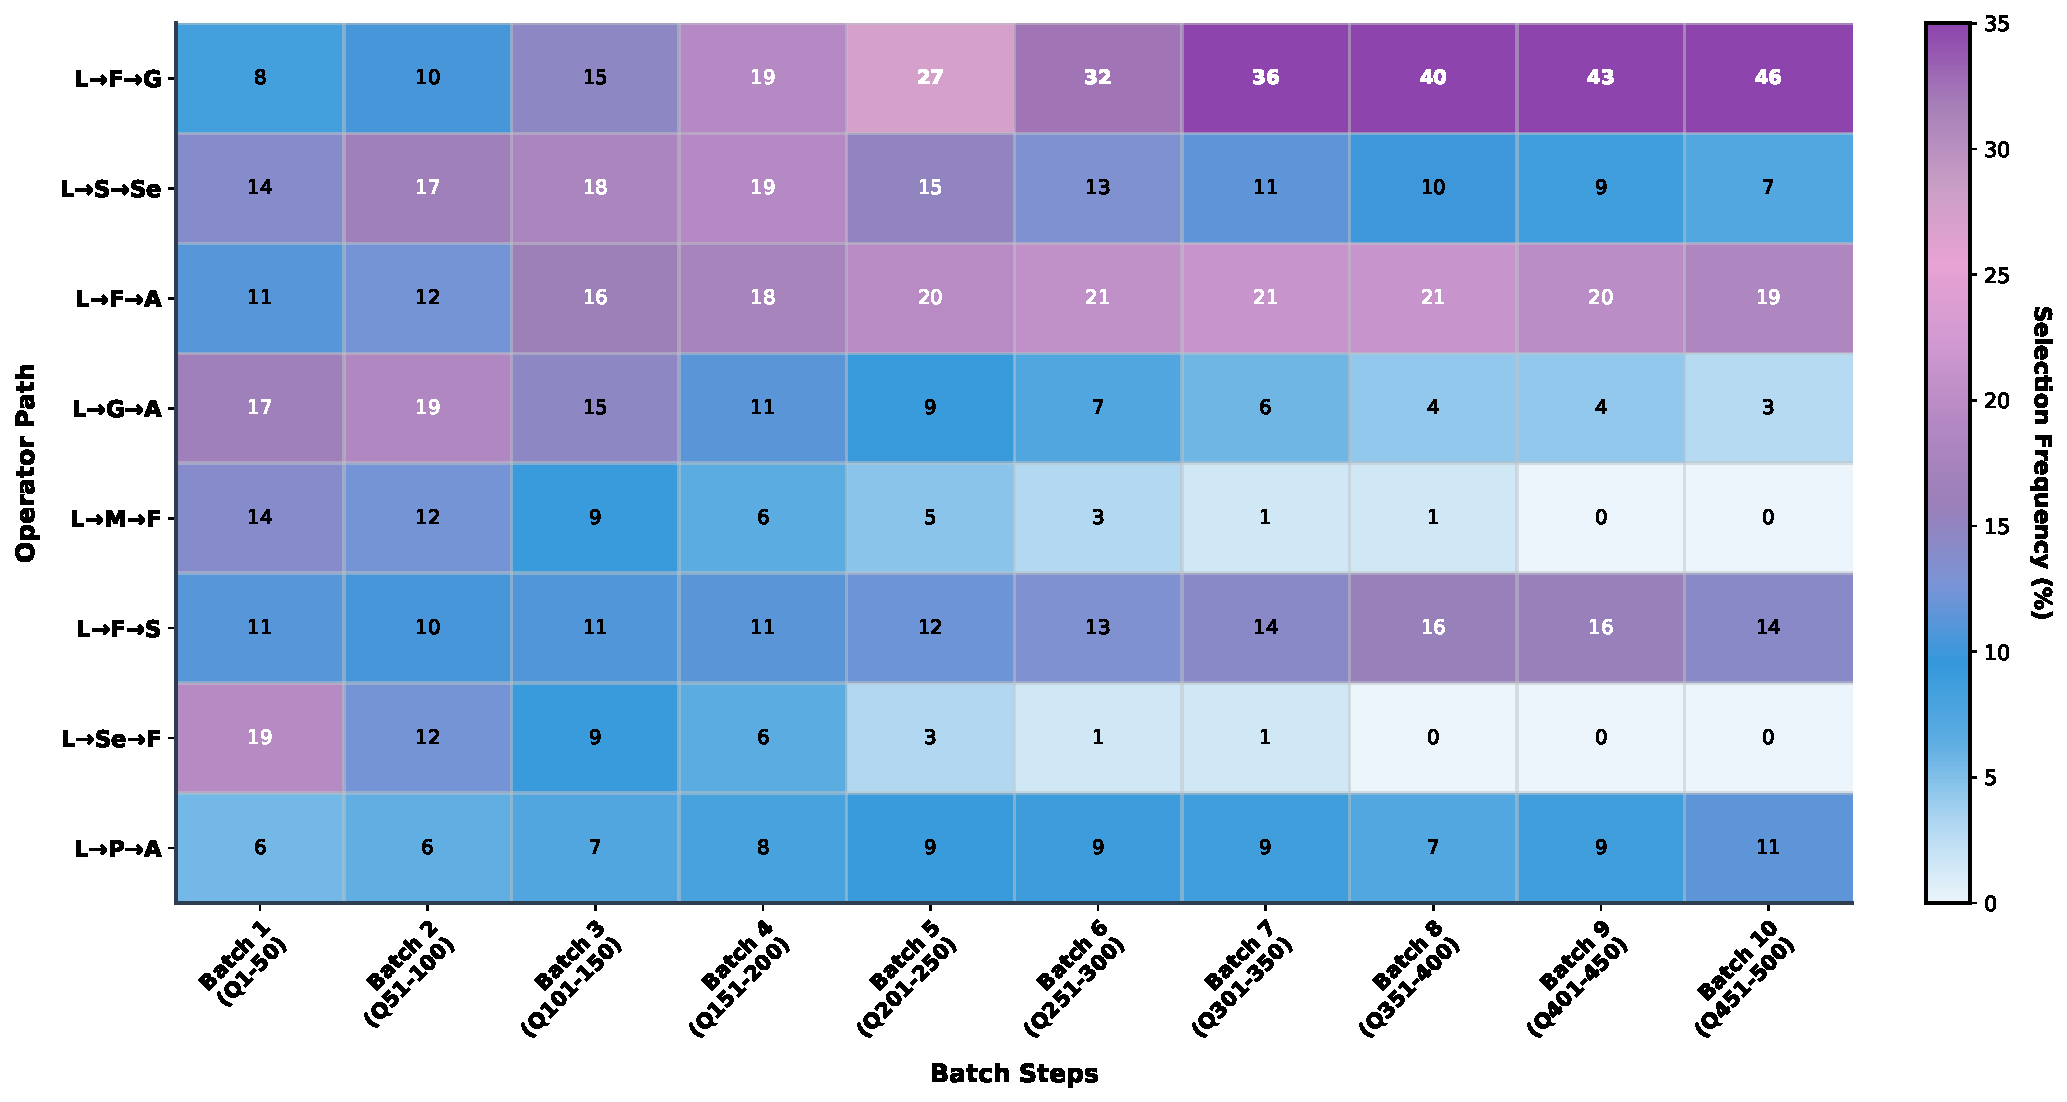
\includegraphics[width=0.92\linewidth]{resources/heatmap.pdf}
    \caption{\footnotesize Path selection evolution across 10 batches. Colors changing from light blue to deep purple indicate  both exploration and exploitation, respectively.}
    \label{fig:path-evolution}
    \vspace{-5mm}
\end{figure}

To further investigate the internal dynamics of DTR, we visualize the evolution of macro path selection over 500 queries partitioned into 10 sequential batches. Figure~\ref{fig:path-evolution} depicts the selection frequency across eight operator paths via a heatmap, where increased density represents higher preference. During the initial batches (1--3), the system engages in broad exploration by selecting candidate paths with near-uniform frequency (3--7\% each). This behavior reflects high initial uncertainty and the necessity of empirical evaluation under diverse tabular conditions.  There exhibits a clear convergence pattern by the fifth batch. Path 0 (\texttt{LOAD} $\rightarrow$ \texttt{FILTER} $\rightarrow$ \texttt{GROUPBY}) increases in frequency from 3\% to 28\%, while paths with consistently low rewards are automatically pruned, e.g., Path 7 which declines to near zero.

Notably, DTR avoids collapsing into a single deterministic strategy. In the final batches (8--10), the primary path stabilizes at roughly 31\% while Path 5 remains a robust secondary option at 11\%. The remaining probability mass is distributed across various alternative paths to maintain approximately 10--15\% exploration. This equilibrium indicates that DTR successfully adapts through execution experience by prioritizing high-return strategies while retaining sufficient diversity for context-sensitive reasoning, demonstrating a balanced exploitation-exploration trade-off.